%%%%%%%%%%%%%%%%%%%%%%%%%%%%%%%%%%%%%%%%%
% Beamer Presentation
% LaTeX Template
% Version 1.0 (10/11/12)
%
% This template has been downloaded from:
% http://www.LaTeXTemplates.com
%
% License:
% CC BY-NC-SA 3.0 (http://creativecommons.org/licenses/by-nc-sa/3.0/)
%
%%%%%%%%%%%%%%%%%%%%%%%%%%%%%%%%%%%%%%%%%

%----------------------------------------------------------------------------------------
%	PACKAGES AND THEMES
%----------------------------------------------------------------------------------------

\documentclass{beamer}

\mode<presentation> {

% The Beamer class comes with a number of default slide themes
% which change the colors and layouts of slides. Below this is a list
% of all the themes, uncomment each in turn to see what they look like.

%\usetheme{default}
%\usetheme{AnnArbor}
%\usetheme{Antibes}
%\usetheme{Bergen}
%\usetheme{Berkeley}
%\usetheme{Berlin}
%\usetheme{Boadilla}
%\usetheme{CambridgeUS}
%\usetheme{Copenhagen}
%\usetheme{Darmstadt}
%\usetheme{Dresden}
%\usetheme{Frankfurt}
%\usetheme{Goettingen}
%\usetheme{Hannover}
%\usetheme{Ilmenau}
%\usetheme{JuanLesPins}
%\usetheme{Luebeck}
\usetheme{Madrid}
%\usetheme{Malmoe}
%\usetheme{Marburg}
%\usetheme{Montpellier}
%\usetheme{PaloAlto}
%\usetheme{Pittsburgh}
%\usetheme{Rochester}
%\usetheme{Singapore}
%\usetheme{Szeged}
%\usetheme{Warsaw}

% As well as themes, the Beamer class has a number of color themes
% for any slide theme. Uncomment each of these in turn to see how it
% changes the colors of your current slide theme.

%\usecolortheme{albatross}
%\usecolortheme{beaver}
%\usecolortheme{beetle}
%\usecolortheme{crane}
%\usecolortheme{dolphin}
%\usecolortheme{dove}
%\usecolortheme{fly}
%\usecolortheme{lily}
%\usecolortheme{orchid}
%\usecolortheme{rose}
%\usecolortheme{seagull}
%\usecolortheme{seahorse}
%\usecolortheme{whale}
%\usecolortheme{wolverine}

%\setbeamertemplate{footline} % To remove the footer line in all slides uncomment this line
%\setbeamertemplate{footline}[page number] % To replace the footer line in all slides with a simple slide count uncomment this line

%\setbeamertemplate{navigation symbols}{} % To remove the navigation symbols from the bottom of all slides uncomment this line
}

\usepackage{graphicx} % Allows including images
\usepackage{booktabs} % Allows the use of \toprule, \midrule and \bottomrule in tables
\usepackage{esint}
\usepackage{listings}

\lstset{frame=none,
	language=c++,
	aboveskip=3mm,
	belowskip=3mm,
	showstringspaces=false,
	columns=flexible,
	basicstyle={\small\ttfamily},
	numbers=left,
	numberstyle=\tiny\color{gray},
	keywordstyle=\color{blue},
	commentstyle=\color{dkgreen},
	stringstyle=\color{mauve},
	breaklines=true,
	breakatwhitespace=true,
	tabsize=4
}

\definecolor{dkgreen}{rgb}{0,0.6,0}
\definecolor{gray}{rgb}{0.5,0.5,0.5}
\definecolor{mauve}{rgb}{0.58,0,0.82}

%----------------------------------------------------------------------------------------
%	TITLE PAGE
%----------------------------------------------------------------------------------------

\title[LLVM JIT]{LLVM Just-in-Time Compiler} % The short title appears at the bottom of every slide, the full title is only on the title page

\author{Rong Yuyang} % Your name
\institute[SIST] % Your institution as it will appear on the bottom of every slide, may be shorthand to save space
{
ShanghaiTech University \\ % Your institution for the title page
School of Information Science and Technology(SIST) \\
\medskip
\textit{rongyy@shanghaitech.edu.cn} % Your email address
}
\date{\today} % Date, can be changed to a custom date

\begin{document}

\begin{frame}
\titlepage % Print the title page as the first slide
\end{frame}

\begin{frame}
\frametitle{Overview} % Table of contents slide, comment this block out to remove it
\tableofcontents % Throughout your presentation, if you choose to use \section{} and \subsection{} commands, these will automatically be printed on this slide as an overview of your presentation
\end{frame}

%----------------------------------------------------------------------------------------
%	PRESENTATION SLIDES
%----------------------------------------------------------------------------------------

%------------------------------------------------
\section{What is JIT} % Sections can be created in order to organize your presentation into discrete blocks, all sections and subsections are automatically printed in the table of contents as an overview of the talk
%------------------------------------------------

%\subsection{Subsection Example} % A subsection can be created just before a set of slides with a common theme to further break down your presentation into chunks

\begin{frame}
\frametitle{What is Just in Time}
\begin{itemize}
	\item Program stored in Bytecode;
	\item Furture compiled right before it's called;
	\item Compilation happens \textit{Just in Time}.
\end{itemize}
\end{frame}

\begin{frame}
\frametitle{Two Engines in LLVM}
	\begin{itemize}
	\item JIT(Old one, to be removed after llvm 3.5);
	\item MCJIT(New one utlizing MC).
	\end{itemize}
\end{frame}

%------------------------------------------------
\section{JIT}
%------------------------------------------------
%------------------------------------------------
\begin{frame}
\frametitle{JIT}
	\begin{itemize}
	\item Function based;
	\item Compile one function at a time;
	\item Compilation happens when function pointer is generated or called(lazy compilation).
	\end{itemize}
\end{frame}

%------------------------------------------------
\begin{frame}
\frametitle{How to use JIT}
	\begin{itemize}
		\item Load \textit{.bc} file;
		\item Construct a parser on the file;
		\item Based on the parser construct an execution engine;
		\item Load one specific function using parser and throw it to the executuon engine;
		\item Woola! You got a function pointer pointing to a newly compiled function;
		\item Call the function.
		\item Release Memory and shutdown llvm
	\end{itemize}
\end{frame}

\defverbatim[colored]\JITCodeOne{
\begin{lstlisting}
	MemoryBuffer::getFile("./sum.bc", Buffer);
	Module *M = ParseBitcodeFile(Buffer.get(), Context, &ErrorMessage);
	OwningPtr<ExecutionEngine> EE(EngineBuilder(M).create());
	Function *SumFn = M->getFunction("sum");
	int (*Sum)(int, int) = (int (*)(int, int)) EE->getPointerToFunction(SumFn);
	int res = Sum(4,5);
	EE->freeMachineCodeForFunction(SumFn);
	llvm_shutdown();
\end{lstlisting}}

\begin{frame}
\frametitle{How to use JIT cont.}
\JITCodeOne
\end{frame}

\begin{frame}
\frametitle{How JIT works}
	\begin{itemize}
		\item Memory Manager: \textit{JITMemoryManager};
		\item Code emitter\textit{$<$Target$>$CodeEmitter};
		\item Target Information(Classes that targets on different platforms \textit{TargetJITInfo})
	\end{itemize}
	\begin{figure}
		\centering
		 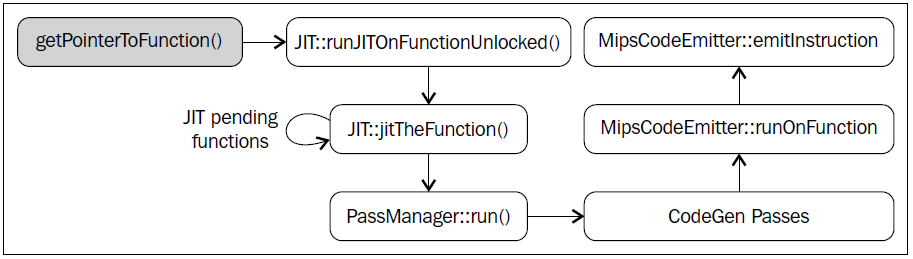
\includegraphics{./pic/flow}
	\end{figure}
\end{frame}
%------------------------------------------------
\defverbatim[colored]\JITCodeTwo{
\begin{lstlisting}
	vector<GenericValue> FnArgs(2);
	FnArgs[0].IntVal = APInt(32,4);
	FnArgs[1].IntVal = APInt(32,5);
	GenericValue Res = EE->runFunction(SumFn, FnArgs);
\end{lstlisting}
}

\begin{frame}
\frametitle{Use of generic value}
\begin{itemize}
	\item Use a \textit{vector$<$GenericValue$>$} as parameters.
	\item Call \textit{runFunction} without getting a function pointer.
\end{itemize}
\JITCodeTwo
\end{frame}

%------------------------------------------------
\section{MCJIT}
%------------------------------------------------
%------------------------------------------------
\begin{frame}
\frametitle{Difference}
\begin{itemize}
	\item Module based. Compilation happens for one module at a time.
	\item Utilizes MC framework we talked in the last Lecture by Zhiqiang.
\end{itemize}
\end{frame}

\begin{frame}
\frametitle{State definition}
\begin{itemize}
	\item Added: Not compiled but already added to the engine;
	\item Loaded: Compiled but not ready for execution;
	\item Finalized: functions executable.
\end{itemize}
\end{frame}

%------------------------------------------------
\section{Discussion}
%------------------------------------------------

\begin{frame}
\frametitle{Interpreter, JIT and Ahead of Time(AOT)}
\begin{itemize}
	\item Interpreter: Shine :)
	\item AOT: C, C++, Rust.
	\item JIT(Somewhere in between): Java, C\#, etc.
\end{itemize}
\end{frame}

\begin{frame}
\frametitle{Pros and Cons}
\begin{itemize}
	\item Pro: Better performance than interpreter.
	\item Pro: Utilizes compile time optimization while using better run-time optimization than AOT
	\item Pro(or Con): Potability. Code once, use(or debug) everywhere.
	\item Con: Translating during run-time takes time(Slow).
	\item Con: Are Readable, Writable and Executable memory pages safe?
\end{itemize}
\end{frame}

%------------------------------------------------
\section{Reference}
%------------------------------------------------
\begin{frame}
\frametitle{Reference}
\begin{itemize}
	\item Getting started with LLVM core libraries.
	\item https://softwareengineering.stackexchange.com/\\questions/246094/understanding-the-differences-traditional-interpreter-jit-compiler-jit-interp
	\item https://www.whizlabs.com/blog/\\what-is-just-in-time-compiler-difference-between-compiler-and-interpreter/
	\item https://stackoverflow.com/questions/95635/what-does-a-just-in-time-jit-compiler-do
	\item https://en.wikipedia.org/wiki/Just-in-time\_compilation
\end{itemize}
\end{frame}
%------------------------------------------------
\end{document} \grid
